%\documentclass[aspectratio=169]
\documentclass[aspectratio=169,xcolor=dvipsnames]{beamer}
%\usetheme{Copenhagen}
\usetheme{Madrid}
\setbeamertemplate{navigation symbols}{}
%\setbeamertemplate{footline}{}
\usecolortheme[named=Green]{structure}

\usepackage[utf8]{inputenc}

\usepackage{graphicx}         
\graphicspath{ {./Pictures/} }
\usepackage{amsmath}
\usepackage{amsfonts}
\usepackage{amssymb}
\usepackage{amsthm}
\usepackage{mathtools}
\usepackage{commath}
\usepackage{multimedia}
\usepackage{subcaption}
\usepackage{media9}
\addmediapath{Animations/}
\newcommand{\Sta}{y}
\newcommand{\Adj}{p}
\newcommand{\Con}{u}
\begin{document}

\title[]{PDE-Constrained Optimization for Multiscale Particle Dynamics}
\author[Jonna Roden]{Jonna Roden}
\institute[UoE]{Joint work with Ben Goddard and John Pearson}
\date{February 12, 2020}

\begin{frame}
\titlepage
\end{frame}
 
 
\begin{frame}
	\frametitle{Structure of the Talk}
	 
	 \begin{itemize}
	 	\item Part 1: What is Multiscale Particle Dynamics?
	 	\item Part 2: What is PDE-Constrained Optimization?
	 	\item Part 3: Numerical Methods and Results
	 \end{itemize}
\end{frame}
\begin{frame}
	\frametitle{Part 1: What is Multiscale Particle Dynamics?}
	
	\begin{columns}
		\column{0.7 \linewidth}	
		What do these pictures have in common?\\
		
		\begin{columns}	
			\column{0.5 \linewidth}
			\begin{figure}
				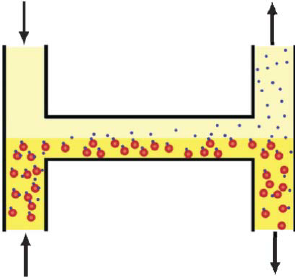
\includegraphics[width=4cm]{Microfilter.png}
				\caption{ Nanofiltration Device}
			\end{figure}
			\column{0.5 \linewidth}
			\begin{figure}		
				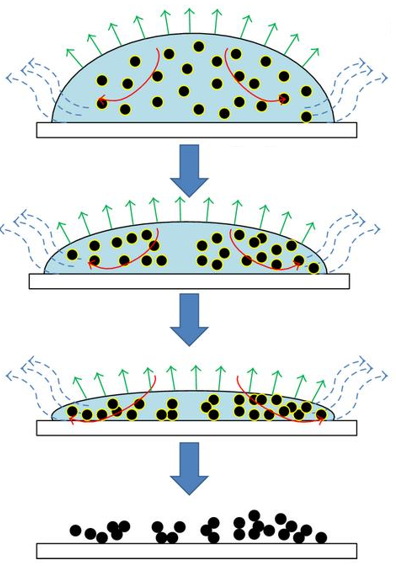
\includegraphics[width=4cm]{printing1.png}
				\caption{Ink Droplet Drying Process}
			\end{figure}
		\end{columns}
		\column{0.3 \linewidth}
		
		\begin{figure}
			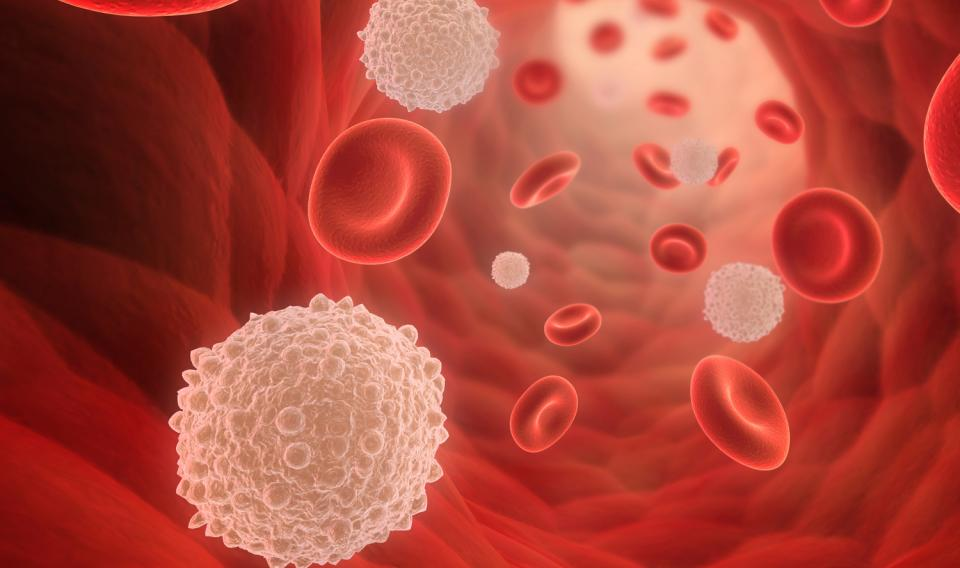
\includegraphics[width=3cm]{bloodcells.jpg}
			\caption{Blood Cells in Blood Vessels}
		\end{figure}
		\begin{figure}
			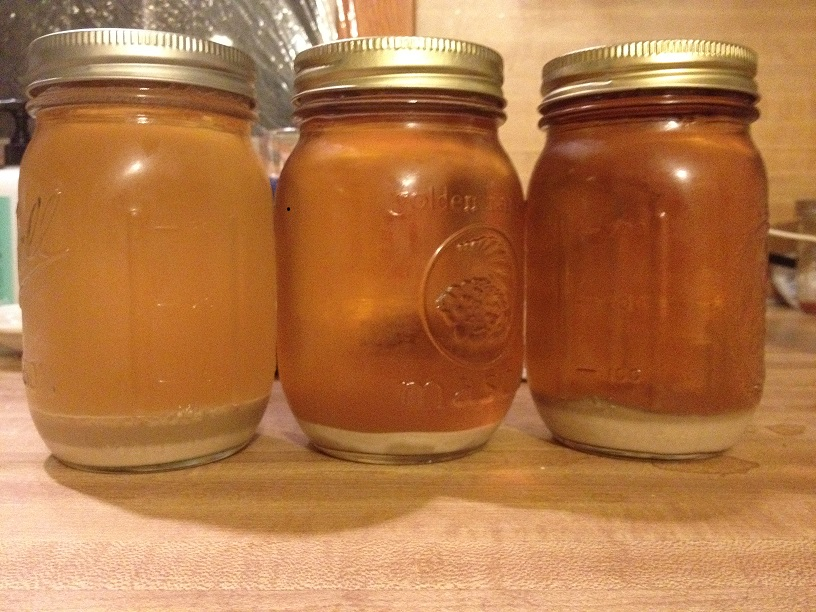
\includegraphics[width=3cm]{beer.jpg}
			\caption{Yeast Sedimentation in Beer}
		\end{figure}
		
	\end{columns}
\end{frame}

\begin{frame}
	\frametitle{Part 1: What is Multiscale Particle Dynamics?}
	 Mathematically, they are like this picture!
	
	\begin{figure}
		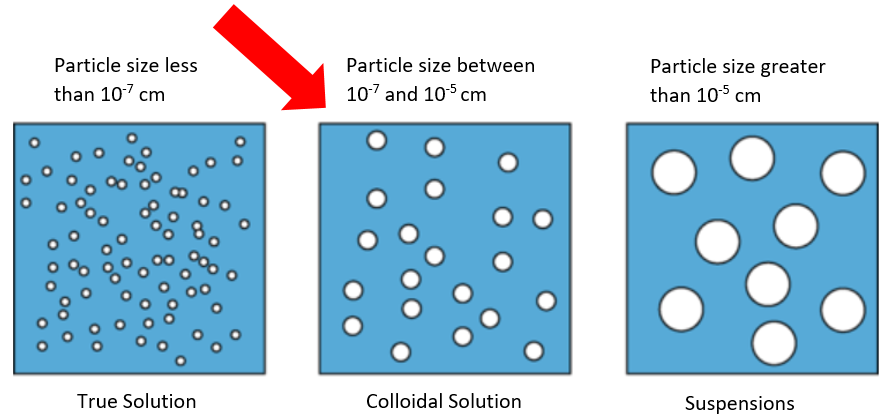
\includegraphics[width=10cm]{Particles2.png}
	\end{figure}
\end{frame}



\begin{frame}
	\frametitle{Modelling of the (Industrial) Process}
	\begin{columns}
		\column{0.8 \linewidth}
		\textbf{Modelling}: Diffusion and Flow
		\begin{align*}
		\rho \text{ is}& \text{ the particle density at } (x,t)\\
		\\
        \partial_t \rho &= \nabla^2 \rho - \nabla \cdot (\rho \mathbf{w}) \qquad \text{in    } \Sigma = \Omega \times (0,T)\\
        \\
        \text{BC }& \text{and IC:}\\
        \frac{\partial \rho}{\partial n}& - \rho \mathbf{w} \cdot \mathbf{n} = 0 \qquad \qquad \text{on   } \partial \Sigma = \partial \Omega \times (0,T)   \\
        \rho(0&,x) = \rho_0(x) 
		\end{align*}
		\column{0.2 \linewidth}
		\begin{figure}
			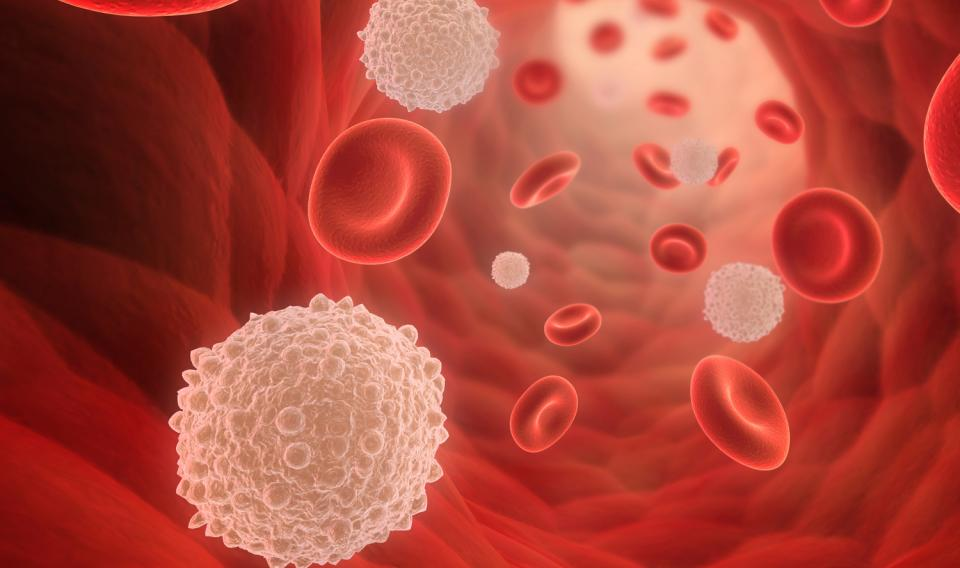
\includegraphics[width=3cm]{bloodcells.jpg}\\
			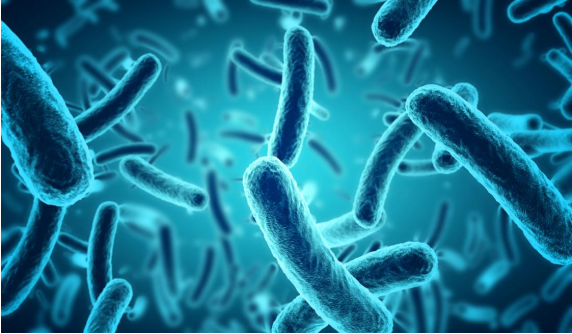
\includegraphics[width=3cm]{bacteria.png}\\
			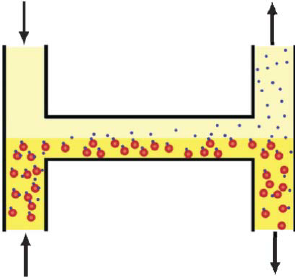
\includegraphics[width=3cm]{Microfilter.png}
		\end{figure}
	\end{columns}
\end{frame}
\begin{frame}
	\frametitle{Modelling of the (Industrial) Process}
	\begin{columns}
		\column{0.8 \linewidth}
		\textbf{Modelling}: Diffusion, Flow and \textcolor{red}{Particle Interactions}
		\begin{align*}
		\rho \text{ is}& \text{ the particle density at } (x,t)\\
		\\
		\partial_t \rho &= \nabla^2 \rho - \nabla \cdot (\rho \mathbf{w}) +\textcolor{red}{ \nabla \cdot \int_\Omega \rho(x) \rho(x') \nabla V_2(|x-x'|)dx'} \qquad\text{in    } \Sigma\\
		\\
		\text{BC }& \text{and IC:}\\
		\frac{\partial \rho}{\partial n}& - \rho \mathbf{w} \cdot \mathbf{n} +\textcolor{red}{ \int_\Omega \rho(x) \rho(x')  \frac{ \partial  V_2}{\partial n}(|x-x'|)dx'} = 0 \quad\ \ \qquad \text{on   } \partial \Sigma   \\
		\rho(0&,x) = \rho_0(x) 
		\end{align*}
		\column{0.2 \linewidth}
		\begin{figure}
			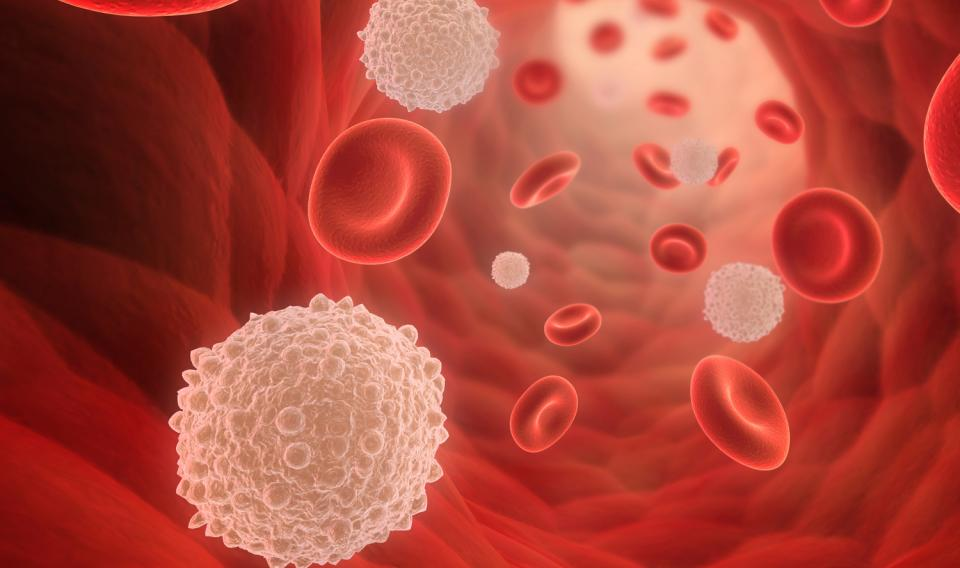
\includegraphics[width=3cm]{bloodcells.jpg}\\
			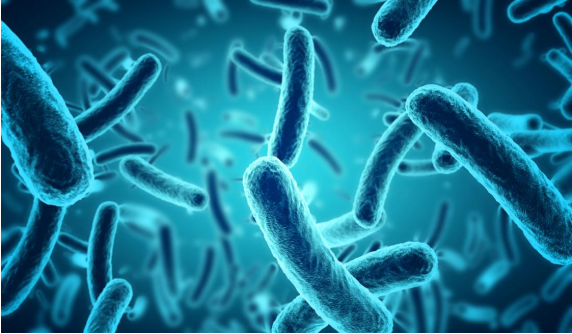
\includegraphics[width=3cm]{bacteria.png}\\
			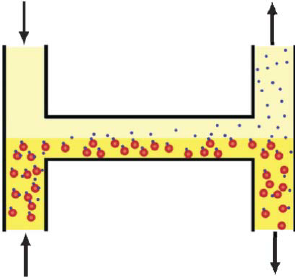
\includegraphics[width=3cm]{Microfilter.png}
		\end{figure}
	\end{columns}
\end{frame}



\begin{frame}
	\frametitle{Part 2: What is PDE-Constrained Optimization? }
	\begin{columns}


		\column{0.6 \linewidth}
		\begin{align*}
		&\min_{\rho,u} \quad \frac{1}{2}\norm{\rho- \hat{\rho}}_{L_2(\Sigma)}^2 + \frac{\beta}{2} \norm{\mathbf{w}}_{L_2(\Sigma)}^2,\\
		\\
		&\text{subject to:}
		\\
		& \partial_t \rho = \nabla^2 \rho - \nabla \cdot (\rho \mathbf{w})\\
		&+\textcolor{red}{\nabla \cdot \int_\Omega \rho(x) \rho(x') \nabla V_2(|x-x'|)dx'} \qquad \text{in    } \Sigma\\
		\\
		&+ \text{BC} + \text{IC}
		\end{align*}
		\column{0.4 \linewidth}
	   \begin{figure}
	    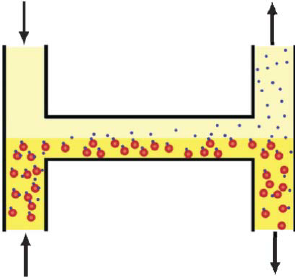
\includegraphics[width=3.5cm]{Microfilter.png}\\
		 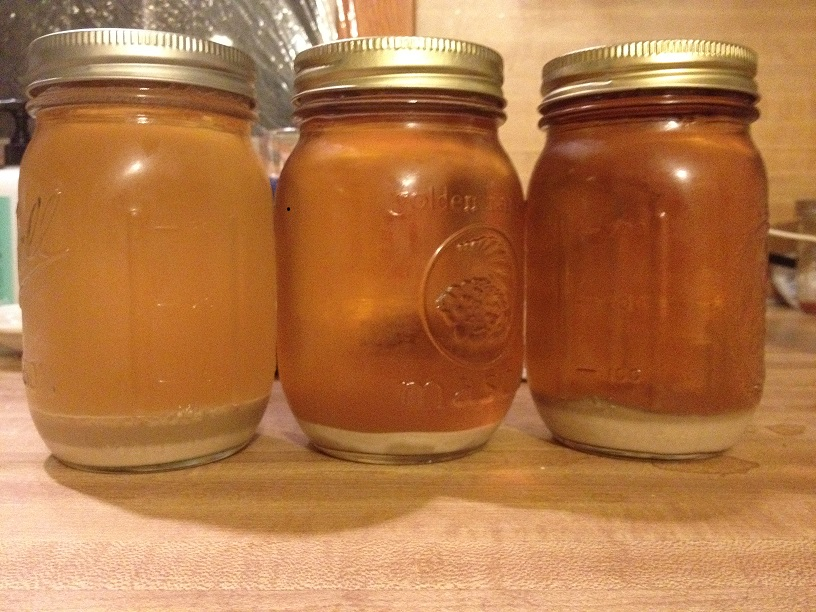
\includegraphics[width=3.5cm]{beer.jpg}
		 \caption{Top: Nano-Filtration Device \\ Bottom: Yeast Sedimentation in Beer}
		\end{figure}
	
	\end{columns}
\end{frame}


\begin{frame}
\frametitle{Optimization of the (Industrial) Process}
\textbf{Deriving (first-order) optimality conditions}\\
Idea: Define the Lagrangian $\mathcal{L}(\rho, \mathbf{w}, q)$:
\begin{align*}
\mathcal{L}(\rho, \mathbf{w},q)&= \frac{1}{2}\norm{\rho- \hat{\rho}}_{L_2(\Sigma)}^2 + \frac{\beta}{2} \norm{\mathbf{w}}_{L_2(\Sigma)}^2\\
&+ \int_\Sigma q \bigg( \partial_t \rho - \nabla^2 \rho + \nabla \cdot (\rho \mathbf{w})
-\textcolor{red}{ \nabla \cdot\int_\Omega \rho(x) \rho(x') \nabla V_2(|x-x'|)dx'}    \bigg) dr dt\\
&+ \int_{\partial \Sigma} q \text{ (BC) } dr dt
\end{align*}
\end{frame}
\begin{frame}
	\frametitle{Optimization of the (Industrial) Process}
	\textbf{Deriving (first-order) optimality conditions}\\
	1. Take derivatives of $\mathcal{L}(\rho, \mathbf{w}, q)$ with respect to $\rho$, $\mathbf{w}$ and $q$. \\
	2. Set derivatives to zero to find stationary points. \\
	\begin{align*}
	 \partial_t \rho &= \nabla^2 \rho - \nabla \cdot (\rho \textcolor{ForestGreen}{\mathbf{w}})
	+ \nabla \cdot \int_\Omega \rho(x) \rho(x') \nabla V_2(|x-x'|)dx'  \\
	\partial_t q &= -\nabla^2 q - \nabla q \cdot \textcolor{ForestGreen}{\mathbf{w}} + \int_\Omega \rho(x') \bigg(\nabla q(x) + \nabla q(x')\bigg)\cdot  \nabla V_2(|x-x'|)dx' \\
    \textcolor{ForestGreen}{\mathbf{w} } \ &\textcolor{ForestGreen}{= - \frac{1}{\beta}\rho \nabla q }\\
    \\
    \rho(0,x)&=\rho_0(x), \qquad q(T,x)= 0 \\
    &+ BC
	\end{align*}
\end{frame}

\begin{frame}
	\frametitle{Optimization of the (Industrial) Process}
     Problem: Negative diffusion term in $q$ causes blowup.\\
     Solution: Rewrite time for this PDE: $\tau = T-t$.
	\begin{align*}
	\partial_t \rho (t,x) &= \nabla^2 \rho (t,x) - \nabla \cdot (\rho(t,x) \textcolor{ForestGreen}{\mathbf{w}(t,x)} )
	+ \nabla \cdot \int_\Omega \rho(t,x) \rho(t,x') \nabla V_2(|x-x'|)dx'  \\
	\partial_\tau q(\tau,x)  &= \nabla^2 q(\tau,x)  + \nabla q(\tau,x)  \cdot \textcolor{ForestGreen}{\mathbf{w}(\tau,x) } \\&- \int_\Omega \rho(\tau, x') \bigg(\nabla q(\tau, x ) + \nabla q(\tau, x')\bigg) \cdot \nabla V_2(|x-x'|)dx' \\
	\rho(0,x)&=\rho_0(x), \qquad q(0,x)= 0 
	\end{align*}
   \begin{figure}
   	\vspace{-0.2cm}
		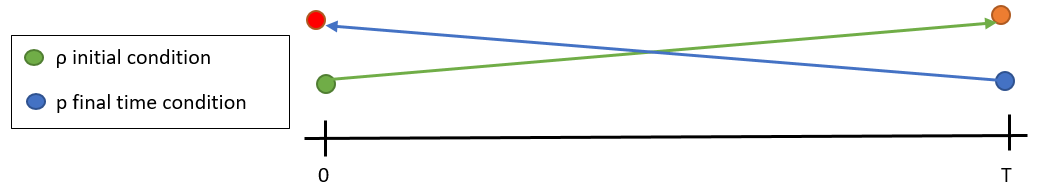
\includegraphics[width=14cm]{FullSol.png}\\
		%\caption{Two Variables}
	\end{figure}
\end{frame}


\begin{frame}
	\frametitle{Part 3: Numerical Methods}
\textbf{Numerics}:\\
 Optimization = Solving the system of PDEs
	\begin{itemize} 
		\item Challenge 1: One PDE is forward in time, the other backward. \\How to do time stepping?
		\item Challenge 2: Particle interaction term is nonlinear and nonlocal (+ nonlocal BCs).
		\item Standard methods (FEM/FDM) are not easily applicable.
	\end{itemize}
We use:
\begin{itemize}
		\item Pseudospectral methods.
		\item Multiple shooting method.
	\end{itemize}
\end{frame}

\begin{frame}
	\frametitle{Part 3: Numerical Methods}
	\textbf{Numerics}: What are pseudospectral methods?\\
	\begin{itemize}
		\item Polynomial interpolation using e.g. Chebyshev nodes.
		\item Discretize space: $\Delta \rho \to D \rho$ (PDE $\to$ ODEs).
	\end{itemize}	
\end{frame}

\begin{frame}
	\frametitle{The Numerical Algorithm}
	\textbf{Numerics}: What is the multiple shooting method?\\
    \begin{itemize}
    	\item Reduce PDE to ODEs using pseudospectral methods.
    	\item Discretize the time interval, guess solution for $\rho$ (and $q$) on each $t_i$.
    	\item Interpolate $q$ between $t_i$ and $t_{i+1}$.
        \item Solve ODE on each time interval, match endpoints.
    \end{itemize}
	\begin{figure}
		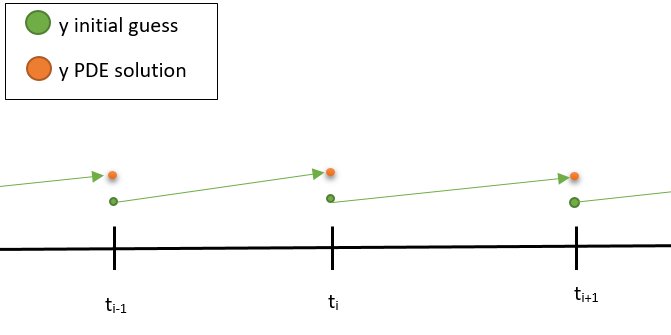
\includegraphics[width=12cm]{rhoSol.png}\\
		\caption{Multiple Shooting}
	\end{figure}	
\end{frame}
\begin{frame}
	\frametitle{The Numerical Algorithm}
	\textbf{Numerics}: What is the multiple shooting method?\\
	\begin{itemize}
     \item Same thing for $q$, but backwards. 
	\end{itemize}
	\begin{figure}
		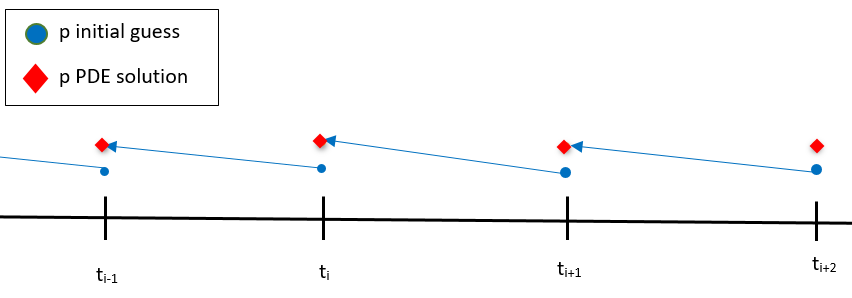
\includegraphics[width=14cm]{qSol.png}\\
		\caption{Multiple Shooting}
	\end{figure}	
\end{frame}
\begin{frame}
	\frametitle{The Numerical Algorithm}
	\textbf{Numerics}: What is the multiple shooting method?\\
   \begin{itemize}
   	\item Create an initial guess for all $\rho$, $q$ on $t_i$.
   	\item Solve both PDEs on subintervals.
   	\item If endpoints don't match, refine initial guess on $t_i$.
   	\item Iterate until endpoints match (within a tolerance) on all $t_i$.
   \end{itemize}
	\begin{figure}
		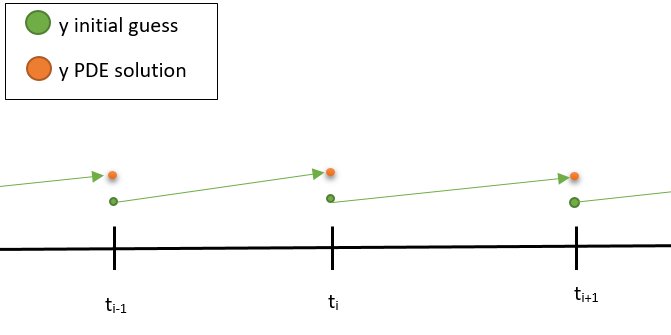
\includegraphics[width=11cm]{rhoSol.png}
	    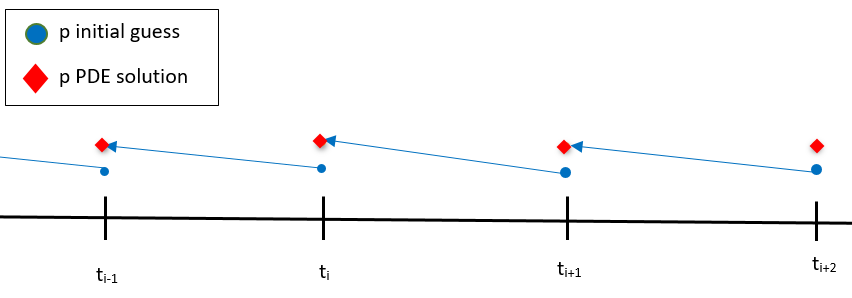
\includegraphics[width=11cm]{qSol.png}
		%\caption{Multiple Shooting}
	\end{figure}	
\end{frame}

\begin{frame}
	\frametitle{A Demonstration of the Numerical Method}
	Overall Cost: $J = \frac{1}{2}\norm{\rho- \hat{\rho}}^2 + \frac{\beta}{2} \norm{\mathbf{w}}^2$
	\begin{columns}	
		\begin{column}{0.5\textwidth} 
			
			$J_{FW}= 1.1930$
			\begin{figure}
				\includemedia[width=0.9\linewidth,height=0.9\linewidth,activate=pageopen,
				passcontext,
				transparent,
				addresource=rhoFW2.mp4,
				flashvars={source=rhoFW2.mp4}
				]{}{VPlayer.swf}
			\end{figure}
		\end{column}
		\begin{column}{0.5\textwidth} 
			$J_{Opt}= 0.8414$
			\begin{figure}
				\includemedia[width=0.9\linewidth,height=0.9\linewidth,activate=pageopen,
				passcontext,
				transparent,
				addresource=rhoOpti2.mp4,
				flashvars={source=rhoOpti2.mp4}
				]{}{VPlayer.swf}
			\end{figure}
		\end{column}
	\end{columns}	
\end{frame}

\begin{frame}
	\frametitle{A Demonstration of the Numerical Method}
	Overall Cost: $J = \frac{1}{2}\norm{\rho- \hat{\rho}}^2 + \frac{\beta}{2} \norm{\mathbf{w}}^2$
	\begin{columns}
		\begin{column}{0.5\textwidth}
			$J_{FW}= 1.1930$ 
			\begin{figure}
				\includemedia[width=0.9\linewidth,height=0.9\linewidth,activate=pageopen,
				passcontext,
				transparent,
				addresource=wFlowFW2.mp4,
				flashvars={source=wFlowFW2.mp4}
				]{}{VPlayer.swf}
			\end{figure}
		\end{column}
		\begin{column}{0.5\textwidth} 
			$J_{Opt}= 0.8414$
			\begin{figure}
				\includemedia[width=0.9\linewidth,height=0.9\linewidth,activate=pageopen,
				passcontext,
				transparent,
				addresource=wFlowOpti2.mp4,
				flashvars={source=wFlowOpti2.mp4}
				]{}{VPlayer.swf}
			\end{figure}
		\end{column}
	\end{columns}	
\end{frame}



\begin{frame}
	\frametitle{Summary}
	We have:
 \begin{itemize}
 	\item Modelled multiscale particle dynamics.
 	\item Solved PDE-constrained optimization problems.
 	\item Used pseudospectral methods and multiple shooting for numerical solutions.
 \end{itemize}
We will:
\begin{itemize}
 	\item Apply this method to industrial processes...
 \end{itemize}
	
\end{frame}
\begin{frame}
	\frametitle{What's next?}
	
	\begin{columns}
		\column{0.5 \linewidth}
		Two industrial partners of the PhD:
		\begin{figure}
			
\includegraphics[width=4cm]{ufraction8.png}
			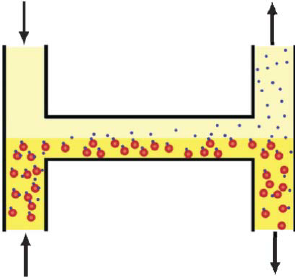
\includegraphics[width=4cm]{Microfilter.png}
			\caption{Nanofiltration Device}
		\end{figure}
		
		\column{0.5 \linewidth}
		\begin{figure}
			
\includegraphics[width=3.5cm]{west.png}\\
			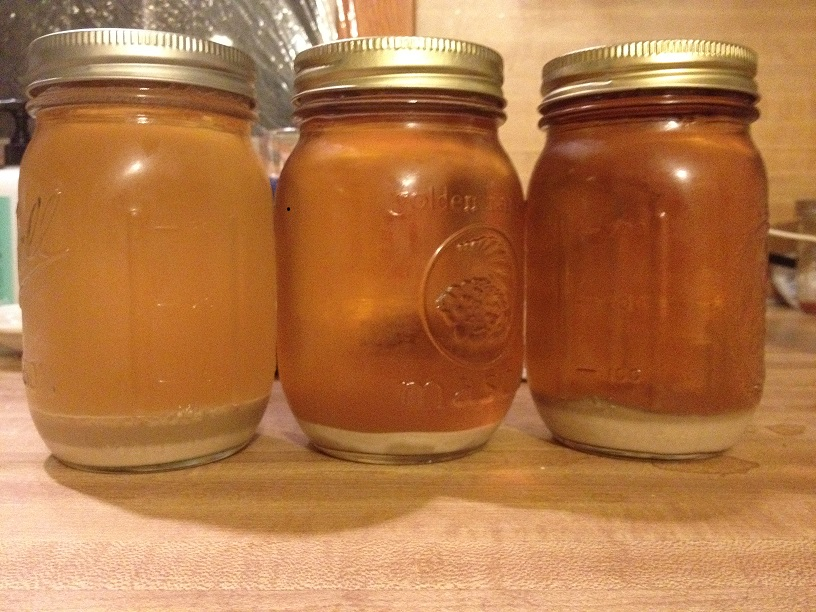
\includegraphics[width=3.5cm]{beer.jpg}
			\caption{Yeast Sedimentation in Beer}
		\end{figure}
	\end{columns}
\end{frame}
\begin{frame}
\frametitle{References}    
\begin{thebibliography}{10}    

	\bibitem{Jemand2000}
     T. Carraro, M. Geiger and R. Rannacher.
	\newblock {\em Indirect Multiple Shooting for Nonlinear Parabolic Optimal Control Problems with Control Constraints.}
	\newblock { \em SIAM Journal on Scientific Computing,} 36(2), 452-481, 2015.
	
	\bibitem{Jemand2000}
	J.C. De los Reyes.
	\newblock {\em Numerical PDE-Constrained Optimization.}
	\newblock 	Springer, 2015.
	
	\bibitem{Autor1990}
	A. Nold, B.D. Goddard, P. Yatsyshin, N. Savva and S. Kalliadasis. 
	\newblock {\em 	Pseudospectral Methods for Density Functional Theory in Bounded and 
		Unbounded Domains}.
	\newblock {\em Journal of Computational Physics}, 334, 639-664, 2017.
	\newblock \url{https://datashare.is.ed.ac.uk/handle/10283/2647} (2DChebClass)
	
\end{thebibliography}
\end{frame}

\begin{frame}
	\frametitle{Part 1: What is Multiscale Particle Dynamics?}
	How can we describe this picture mathematically?\\
	\vspace{1cm}
	\begin{columns}
		\column{0.3 \linewidth}
		
		\begin{figure}
			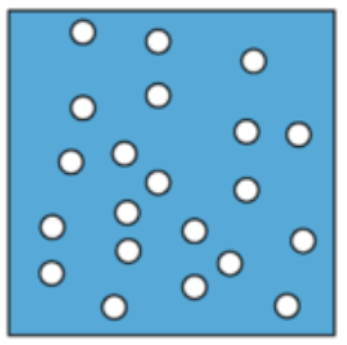
\includegraphics[width=4cm]{Particles3.png}
		\end{figure}
		\column{0.7 \linewidth}
		On Multiple Scales:
		\begin{itemize}
			\item Experimentally \textcolor{red}{(expensive in cost and time!)}
			\item ODEs for $N$ particles AND $n$ water molecules\\ \textcolor{red}{(expensive computations!)}
			\item SDEs for $N$ particles \textcolor{red}{(expensive computations!)}
			\item PDEs for the $N$ particle density  \textcolor{red}{(impossible computations!)}
			\item PDEs for the $1$ particle density \textcolor{green}{(good compromise)}
			\item PDEs for the bulk fluid \textcolor{red}{(inaccurate for many processes!)}
		\end{itemize}
	\end{columns}
\end{frame}
\begin{frame}
	\frametitle{Modelling of the (Industrial) Process}
	\begin{columns}
		\column{0.8 \linewidth}
		\textbf{Modelling}: What can we describe with our PDEs?
		\begin{itemize}
			\item Forces
			\item Particle Interactions
			\item Multiple Species
			\item Self-Propelled Particles
			\item Different Geometries
			\item ...
		\end{itemize}
		\column{0.2 \linewidth}
		\begin{figure}
			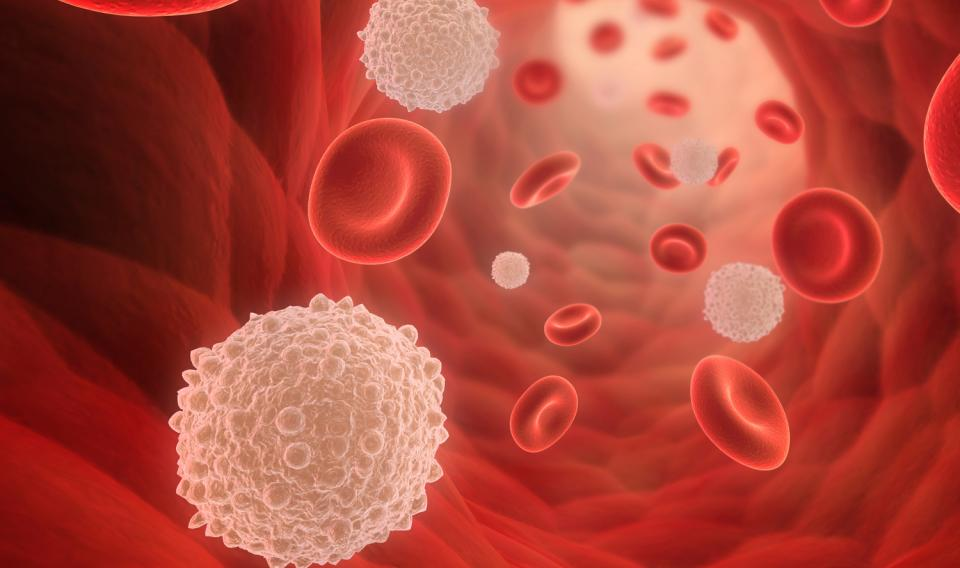
\includegraphics[width=3cm]{bloodcells.jpg}\\
			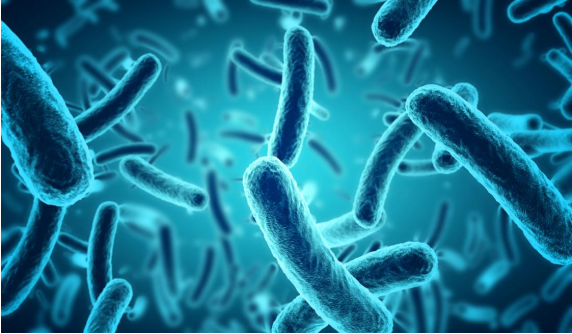
\includegraphics[width=3cm]{bacteria.png}\\
			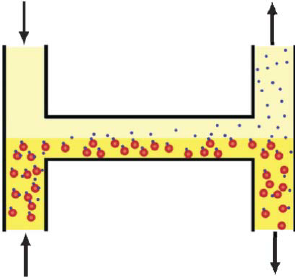
\includegraphics[width=3cm]{Microfilter.png}
		\end{figure}
	\end{columns}
\end{frame}
\begin{frame}
	\frametitle{Numerical Methods}
	\textbf{Numerics}: What are pseudospectral methods?\\
	\begin{itemize}
		\item Polynomial interpolation using e.g. Chebyshev nodes.
		\item Discretize space: $\Delta \rho \to D \rho$ (PDE $\to$ ODEs).
	\end{itemize}
	
	
	\begin{figure}
		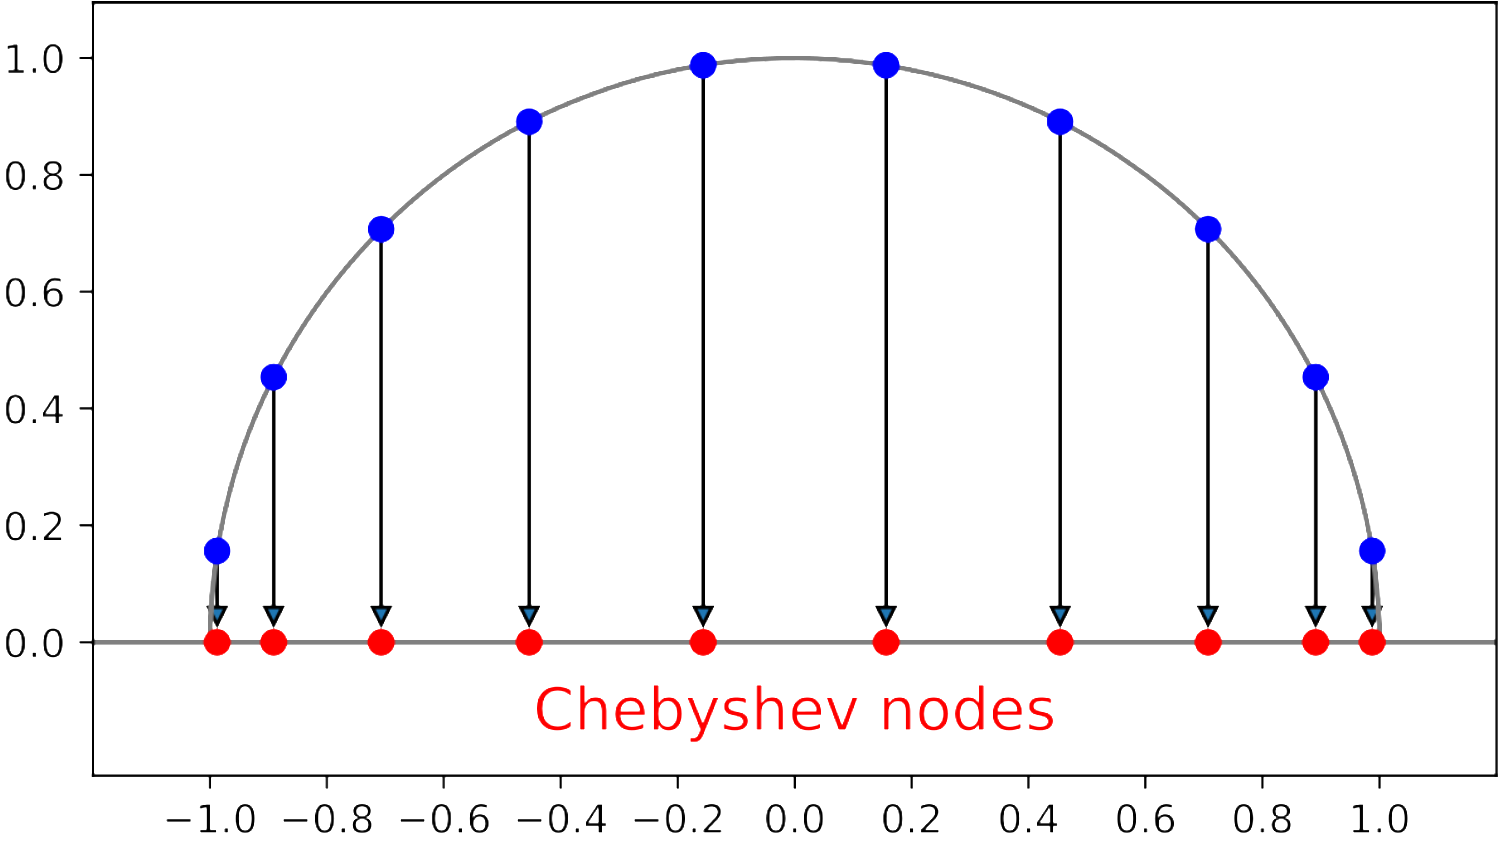
\includegraphics[width=8cm]{chebnodes1.png}\\
		%\caption{Chebyshev nodes}
	\end{figure}	
\end{frame}

%By SunKart at English Wikipedia, CC BY 3.0, https://commons.wikimedia.org/w/index.php?curid=17582614 colloid picture
\end{document}